

\lettrine[lines=3]{T}{}he motion of plants is an important factor when looking to create realistic looking plant-life. It has been a topic of discussion and research for many years now, particularly with regards to grass, bushes and trees within video games. The movement is usually very subtle, but if it is missing, a scene can start looking very unnatural, making the user feel uncomfortable. This chapter will discuss a method of simulating the physical motion of plant-life, layed out by Barron et al \cite{barron2001real}. This method will be built into the parametric L-system itself in such a way that the L-system can provide the physical parameters for the simulation. This will allow a physics simulation to be run on any plant generated by the L-system.

The main technique discussed by Barron et al for simulating the motion of a system like a tree or plant, is taken from that of a particle system, first described by Reeves \cite{reeves1983particle}. Particle systems can be applied to simulate phenomena like clouds, smoke, water and fire. The main advantage of particle systems is that the motion for each particle can be updated simaltaniously. This technique can be applied to the L-system representation of plant-life. Where branches are split into segments that make up a skeleton of segments or joints. Each joint can represent a \say{particle} within the system, which has a dependency on all of its parent branches.

Using the particle system concept, the motion of the plant can simulated by having each joint within the plant skeleton to be seen as a particular segment of a branch with some basic physical properties. These properties include but are not limited to the width, length, direction vector, spring consistant and dampening constant. The direction vector is the global direction of the branch in 3D space pointing in the direction that the branch itself is pointing. The spring constant and the dampening constant are used for Hook's Law. The spring force of the branch tries to prevent it from bending. Whereas gravity, wind and other forces cause torque, which generally acts against this spring force, causing the branch to bend.

\section{Branch Physical Properties}

The mass of each branch segment can be simply calculated by taking the volume of each branch and multiplying it by the density of the wood or material. To do this the volume of each branch needs to be calculated. This can be done by multiplying $\pi$ by the radius $r$ squared and the length $l$ as sees below.

\begin{equation}
v  = \pi r^2 l
\end{equation}

\noindent
This is not always the case, particularly if the branch segment is decreasing in size, however it gives a good inidication as to volume. This can now be used to calculate the mass, this requires knowing the density of the material that the plant is made of. For instance the density of pine wood is between 400 - 420 $\text{kg/m}^3$. Some woods being less dense at about 200 $\text{kg/m}^3$, and other hard wood being up to about 1000$\text{kg/m}^3$.

\begin{equation}
m = v \times d
\end{equation}

\noindent
The mass can be used to calculate the branch segments moment of inertia, this being the branches resistance to angular momentum. As the object is 3D the shape of the object needs to be taken into account. Each branch can be simply seen as a long thin cylinder, which can be expressed in the following equation.

\begin{equation}
I = \frac{1}{3} m l ^ 2
\end{equation}

\noindent
Where $I$ is the inertia of the branch, $m$ is the mass of and $l$ is the lenght. Similarly an inertia tensor can be used for the sake of convenience and to better describe the objects rotational inertia which is used within vector and matrix calculations. The intertia will be used when calculating the velocity of each segment in section \ref{motion equations}. Below is an inertia tensor for a shape that is similar to that of a branch segment.

\begin{equation}
\begin{aligned}
I = \begin{bmatrix}
\frac{1}{12}m(3r^2 + l^2) 	& 0 							& 0 \\
0 							& \frac{1}{12}m(3r^2 + l^2)		& 0 \\
0 							& 0 							& \frac{1}{2}mr^2 
\end{bmatrix}
\end{aligned}
\end{equation}

\noindent
The forward vector of the branch, this being the vector in the direction that the branch is pointing towards, can be used to calcuate the direction the torque is acting on the branch $V$, by taking the cross product of the forward vector $v$ and the force vector $w$. This can be visualised using the right hand rule, where the index finger is the forward vector and the middle finger is the force vector. The direction of the thumb then points in the direction of the torque. The angular velocity is produced as spin in the direction around the torque vector.

\begin{equation}
V = v \otimes w
\end{equation}

\noindent
The dispacement can be calculated by keeping track of the starting local rotation of the branch $p$ as well as the current rotation of the branch $q$ in the form of two quaternions. We can then calculate a quaternion $d$ for the differece of the two quaternions, by taking $p$ and multiplying it by the inverse of $q$. 

\begin{equation}
d = p \times q^{-1}
\end{equation}

\section{Hook's Law}

Hook's law is a law of physics that states that the resultant force from compressing or extending a spring is equal to the product of the spring constant and the displacement of the spring. Each branch in a plant structure can be seen as a type of semi-rigid spring where external forces like gravity or wind bend the spring. Hook's law is used to then calculate the reaction force due to the displacement of the spring.

\begin{equation}
f = -k _s d + k _d v
\end{equation}

\noindent
Where $f$ is the force exerted by the spring, $k _s$ is the spring constant and $x$ is the total displacement of the spring. The dampening force can be calculated as $k _d v$ part where $k _d$ is the dampening constant and $v$ is the velocity at the end of the spring. 


\section{Equations of Motion} \label{motion equations}

The forces can then be multiplied together to get the net force $f_net$ acting on the spring, this can be used to calculate the momentum and furthermore the velocity of the the branch. $T_{delta}$ is that change in time between physics calculations.

\begin{equation}
M = M_0 + f_{net} * T_{delta}
\end{equation}

\noindent
The velocity $v$ can be calculated by taking the inverse of the inertia tensor $I$ and multiplying that by the momentum vector $M$.

\begin{equation}
v = I^{-1} * M
Q_v = [0, v]
\end{equation}

\noindent
The velocity vector can be converted to its quaternion form $Q_v$ in order to make the last step simpler. The scalar part of quaternion can be set to 0 and the vector part can be set to $v$. This allows the next rotation quaternion $R$ to be calculated. 

\begin{equation}
R = R_0 + (\frac{1}{2} * Q_v * R_0 * T_{delta})
\end{equation}

\noindent
Where $R$ is the next local rotation quaternion, $R_0$ is the previous local rotation quaternion, $Q_v$ is the velocity quaternion and finally $T_{delta}$ is the change in time since the previous physics update. This new rotation quaternion can then replace the current local rotation of the branch in turn simulating the motion of the branch.

\section{Updating Branches}

The particles in this system are the joints within the trees' skeleton. All of these joints have to be updated in each update step. This can happen as frequently as needed. A consideration is that if the branches aren't updated frequently enough the animations will not look smooth. Effectively each update step needs to take the forces acting on each branch, its current position and rotation and then calculate the next position and rotation of that branch. This information is then used to generate the model of the tree once again. This is passed to the renderer which will render the result. 

\section{Results}

\begin{figure}[htbp]
	{\centering
		\vspace{7px}
		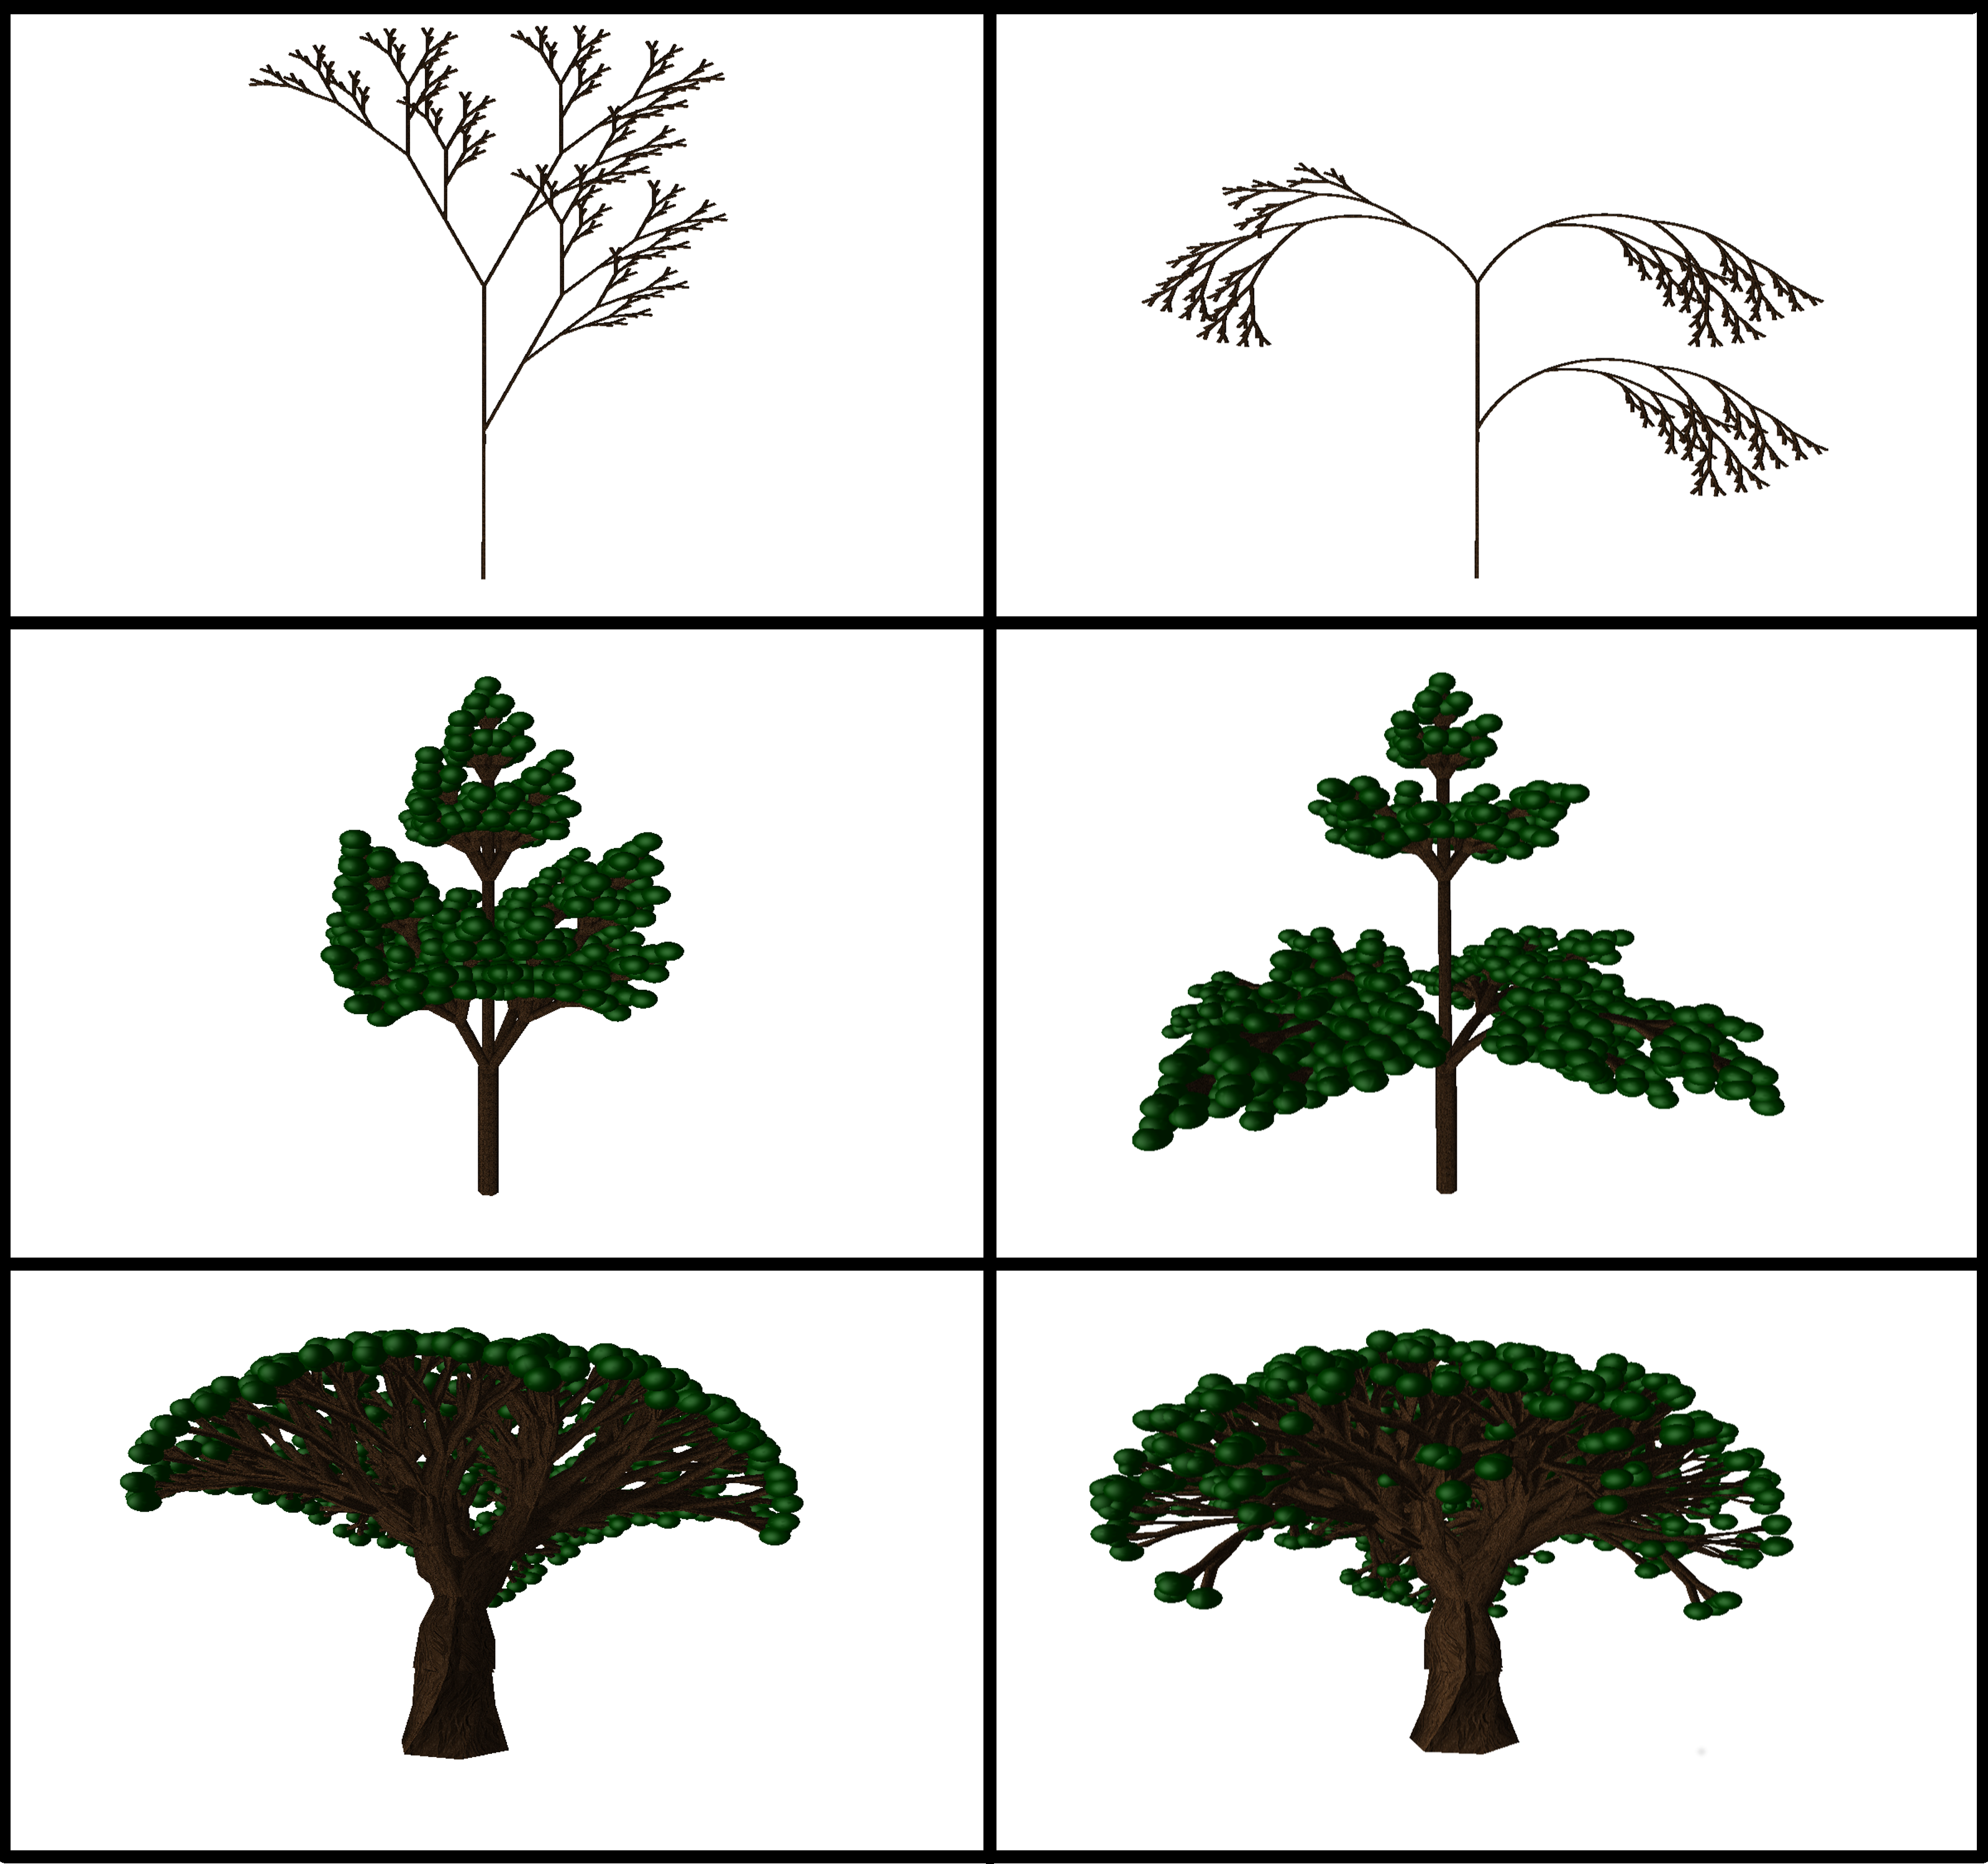
\includegraphics[scale=0.1]{Diagrams/gravityExamples.png}
		\label{3DAxisFigure} \label{Gravity applied to generated models}
		\caption{Examples simulating gravity on different 3D models}
	}
\end{figure}
\FloatBarrier

\section{Summary}

This chapter outlined a method of simulating and animating a procedurally generated plant-life by representing each branch as a  particle in a larger particle system. The information about the location, rotation, dimensions and properties of each branch is provided by the tree skeleton created during the interpretation stage which is ultimately provided by the L-system. Using these properties each branch can be simulated as a particle within the entire tree system. Due to the embarrassingly parrallel nature of the system each branch update can be computed in parallel, either on the \acrshort{cpu} or \acrshort{gpu}.    

